\subsection{Motivation}
A cut-based top jet tagger is applied for the analysis of the 2015 data\cite{CMS-PAS-SUS-16-030}. The cut-based top jet tagger has a good efficiency over the top quark $p_{T}$ spectrum. However, the mistag rate, i.e., the rate at which an object that is not a top quark is erroneously tagged as such by the top tagging algorithm, is relatively high with this algorithm. Therefore, we designed a new top tagger, to reduce the mistag rate. 

\subsection{Description of the method}
\label{sec:toptagger}

Before discussing the top tagging algorithm, we review the top decay modes. Top quark decays (Fig~\ref{fig:c4twdecaymod}) can be categorized into two classes: hadronically decaying top quarks and leptonically (and semi-leptonically) decaying top quarks. We focus on the hadronically decaying top quark since we are searching SUSY in hadronic channels. From the point of view of their reconstruction, hadronic top quark decays can be divided into three categories (Fig~\ref{fig:c4twdecaymod}): a fat mono-jet with a mass close to the top quark, di-jet event containing one fat jet with a mass close to the W boson mass and one tagged b-jet, and a tri-jet event with three jets. The cut-based algorithm is designed following these three scenarios. 

\begin{figure}[htbp]
 \begin{center}
  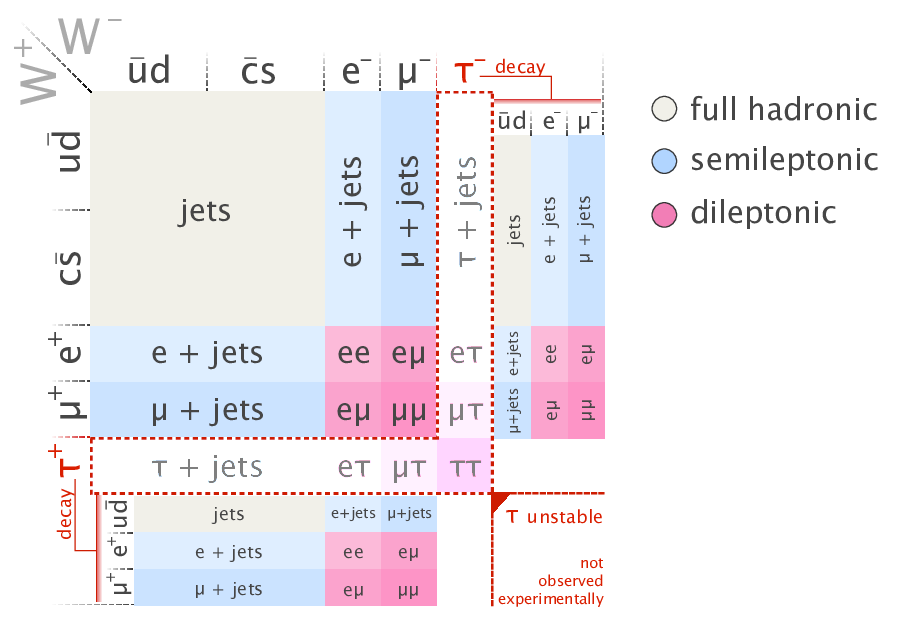
\includegraphics[width=0.55\textwidth]{figures/c4/c4_top_w_decaymod.png}
  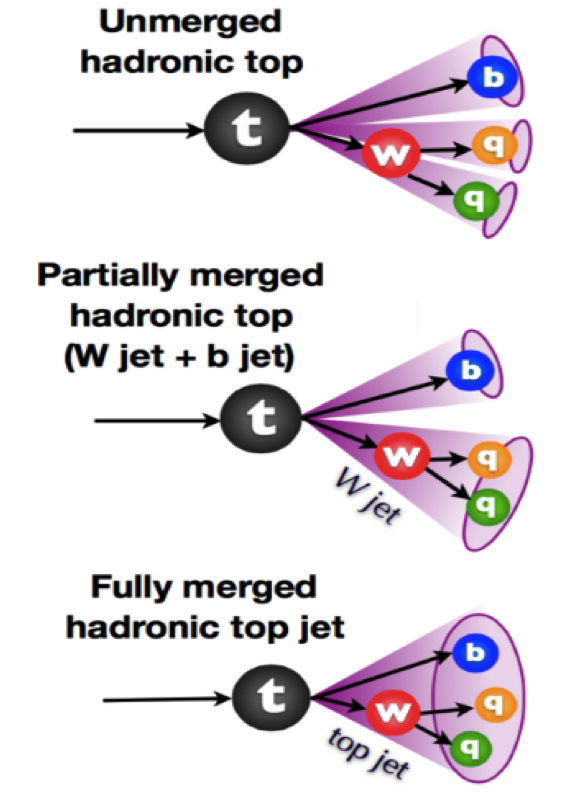
\includegraphics[width=0.25\textwidth]{figures/c4/c4_tagger_hadtopdecay.png}
 \end{center}
 \caption{Left: \ttbar events final states; Right: Hadronically decayed tops}
 \label{fig:c4twdecaymod}
\end{figure}

Only the small AK4 cone jet collection is used in the cut-based tagger in order to simplify the procedure. A negative side effect of this choice is that the remnant system can be relatively large in the mono-jet and di-jet cases. The cut-based algorithm is not very powerful for the tri-jet system, compared with multivariate algorithms. Therefore, the new top tagger has two major upgrades: fat jets (AK8 jet) for the mono-jet and di-jet top systems, and a multivariate algorithm for the tri-jet system. We expect a lower mistag rate with the similar top quark tagging efficiencies after the upgrade. 

The mono-jet top selection is relatively simple. The requirements for the mono-AK8 jet are:
\begin{itemize}
\item AK8 jet $p_{T}\ge$400 GeV.
\item Soft drop mass\cite{Larkoski:2014wba} between 105 and 210 GeV. The soft-drop algorithm reclusters the AK8 jet into subjet using the Cambridge-Aachen algorithm\cite{Dokshitzer:1997in}. The soft radiation is removed to avoid the bias on jet mass determination.
\item N-subjettiness $\tau_{32}\le$0.65. The N-subjettiness is defined in Eq~\ref{eq:c4nsubjettiness}:
\begin{equation}
 \tau_{N}=\frac{1}{d_{0}}\sum_{k} p_{T,k}min{\Delta R_{1,k},\Delta R_{2,k},...,\Delta R_{N,k}}
 \label{eq:c4nsubjettiness}
\end{equation}
, where $\Delta R_{N,k}$ is the angular separation between constituent k and candidate subjet N. $d_{0}$ is a normalization factor given by: $d_{0}=\sum_{k}p_{T,k}R_{0}$, $R_{0}$ is 0.8 for AK8 clustering. The $\tau_{32}=\frac{\tau_{3}}{\tau_{2}}$. Rejecting events with $\tau_{NM}$ close to 1 selects for jets that are more N-prong like\cite{Cohen:2012yc}. Therefore, three-prong like AK8 jets are selected with this requirement.
\end{itemize}

If an AK8 jet is tagged as a top quark for the mono-jet case, it will be removed from the jet collection for di-jet and tri-jet case. 

We require one W-like AK8 jet and b-like AK4 jet in the di-jet case. The W-like AK8 jet is selected with following requirements:
\begin{itemize}
\item AK8 jet $p_{T}\ge$200 GeV.
\item Soft drop mass between 65 and 100 GeV.
\item N-subjettiness $\tau_{21}\le$0.60. Two-prong like AK8 jets are selected with this requirement.
\end{itemize}

Then, the W-like AK8 jet is combined with an AK4 jet with $p_{T}\ge$40 GeV. The additional requiremnets on the di-jet system is:
\begin{itemize}
\item di-jet system mass is between 100 to 250 GeV.
\item the two jets in the di-jet system both lie in a cone of radius R=1.0 centered on the direction of their summed $p_{T}$ vector.
\item jet mass ratio between AK8 W-like jet and di-jet system in range $[ 0.85 \frac{m_{W}}{m_{t}}, 1.25 \frac{m_{W}}{m_{t}} ]$, where $m_{W}$ and $m_{t}$ are the nominal W boson and top quark masses, respectively.
\end{itemize}

We design an overlap remove algorithm to avoid double counting jet energy in the algorithm. An AK4 jet is consideredmatched if it lies within $\Delta R <$ 0.4 of one of the soft-drop subjets of the tagged AK8 jet.

A multivariate analysis is applied to separate signal top quarks from background for candiates in the trijet category. There are two key elements in the multi-variable algorithm design: input variables and the algorithm itself. 

%FIXME

To identify a top quark jet, we have two set of variables for choice. The first set is on the particle candidate level. The $p_{T}, \eta, \phi$ can be used as training variables. However, there are about 400 particle-flow candidates in the tri-jet cone (R=1.5). The convolutional neural network\cite{NIPS2012_4824} (CNN) might be a good algorithm to deal with the classification problem with that amount of features in one top quark candidate. However, the CNN training is very time consuming and it is not a commonly used method in experimental high-energy physics for now. Therefore, we choose the second set: three-jet combination. There are only about 10 features per event, therefore relatively quick to be trained with a decision based algorithm. Several multivariate algorithms are applied on the simulation sample. The random forest algorithm\cite{Ho:1995:RDF:844379.844681} is used as the identification algorithm.

%In general, we have two input variables types: the high-level physics variables, like jet $p_{T}$, and base level physics variable, like particle flow candidate, and calorimeter pixels. The algorithm choosing is dependent on the input variables. For example, the high-level variables are more suited for the decision tree based algorithm, while base level variables prefer neutral network. 
%We choose the high-level physics variables and decision tree based algorithm in our analysis. 

All three-jet combinations are potential top quark candidates. The following variables are considered in the algorithm: 
\begin{itemize}
\item Top quark candidate properties: mass, $p_{T}$, R cone size.
\item Constituent jet properties: jet $p_{T}$, $\eta$, $\phi$; CSV value (b-tag likelyhood), quark-gluon discriminator.
\item Angular variables between jets: $\Delta \phi, \Delta \eta, \Delta R$.
\end{itemize}

All the variables are carefully studied before being used to train the decision tree. Let’s use the quark gluon discriminator as an example. Because of its larger color charge, gluon jets radiate more, leading to a larger particle multiplicity, a broader $p_{T}$ spectrum of its emitted particles with respect to the jet axis, and a softer energy spectrum of the emitted particles. The quark gluon discriminator is a likelihood method used to separate quark and gluon jets. A likelihood value near 1 means it is more like a quark jet, and otherwise that it is more like a gluon jet. We expect top tagger mistag rate to be reduced after incorporating the quark-gluon discriminator into the decision tree since gluon jets, which tend to be fat, can be similar to the fat jets used in the mono-jet and di-jet top quark reconstruction categories. The likelihood is constructed from three variables: 
\begin{itemize}
\item $p_{T}D$: jet energy dispersion variable, defined as $p_{T}D=\frac{\sqrt{\sum_{i}p_{T,i}^{2}}}{\sum_{i}p_{T,i}}$, with sum over all PF candidates. The quark jets are usually have a higher $p_{T}D$ than the gluon jets.
\item Mutiplicity: the total number of particle-flow candidates in the jet. On average, gluon jets have a higher mutiplicity than quark jets.
\item Axis2: minor axis RMS in the $\eta - \phi$ plane of the particle flow candidates. This is an angular spread for the jet. The gluon jets are usually more sparse than the quark jets.
\end{itemize}

The multivariate algorithm does a better job to evaluate the correlations between training variables than cut-based method. To determine the performance of the quark gluon discriminator on different jet flavors, $p_{T}$ and $\eta$, we studied the following jet flavors in \ttbar simulation samples: light flavor jet, c-jet, b-jet, gluon jet and pile-up jet. The $p_{T}$ and $\eta$ schemes are listed in Table~\ref{tab:c4ttqgl}.

\begin{table}[htbp]
\fontsize{10 pt}{1.2 em}
\selectfont
\begin{centering}
\caption{\label{tab:c4ttqgl} Jet bin for quark-gluon discriminator study}
\hspace*{-4ex}
\begin{tabular}{|c|c|c|c|c|c|c|}
\hline
Jet $\eta$ Bin  & \specialcell{1,\\HB} & \specialcell{2,\\HBHE} & \specialcell{3,\\HE} & \specialcell{4,\\HEHF} & \specialcell{5,\\HF} & \specialcell{6,HF \\no PDF} \\
\hline
Jet $\eta$      & [0,1.31] & [1.31,1.39] & [1.39,2.65] & [2.65,3.14] & [3.14,4.7] & [4.7,5.19] \\
\hline
Jet $p_{T}$ Bin & \specialcell{1,\\no PDF} & 2 & 3 & 4 & 5 & 6 \\
\hline
Jet $p_{T}$     & [0,20] & [20,40] & [40,50] & [50,80] & [80,100] & [100,Inf] \\
\hline
\end{tabular}
\par\end{centering}
\end{table}

The performance in terms of jet $\eta$ in different jet flavors is shown in Fig~\ref{fig:c4ttqgljeteta}. The discrimination power for low $p_{T}$ jets is not ideal. 
\begin{figure}[htbp]
 \begin{center}
  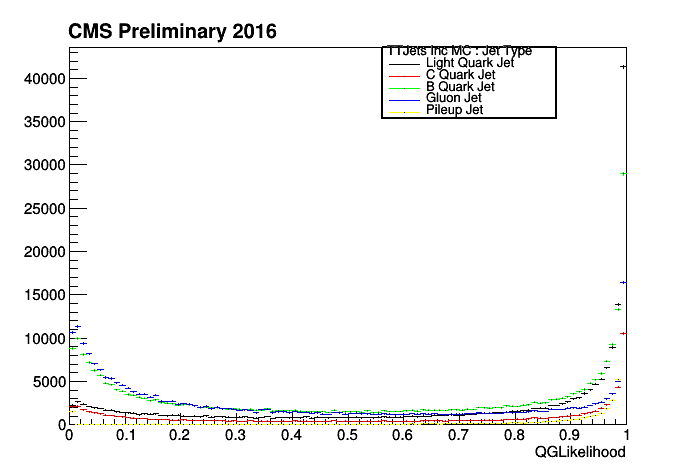
\includegraphics[width=0.45\textwidth]{sections/mc4/TopTagger/figures/_b_qglikelihoodjetetabin0_.png}
  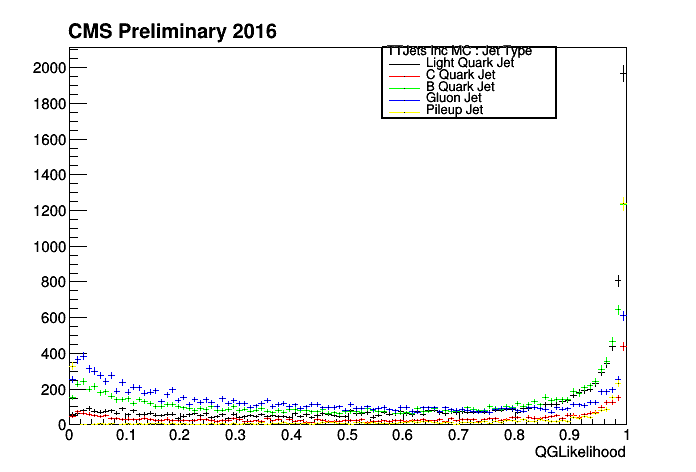
\includegraphics[width=0.45\textwidth]{sections/mc4/TopTagger/figures/_b_qglikelihoodjetetabin1_.png} \\
  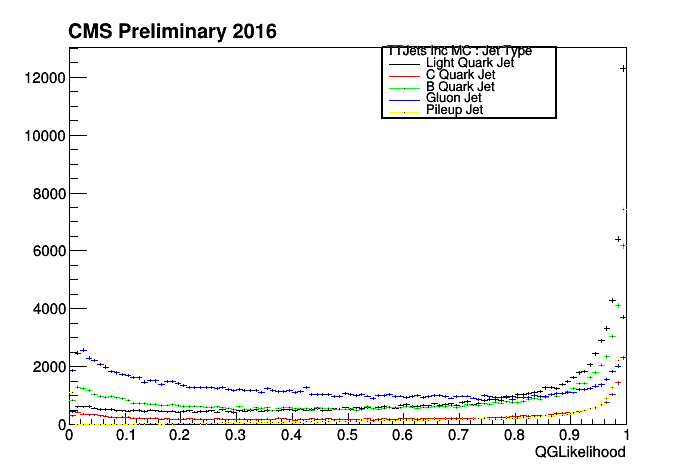
\includegraphics[width=0.45\textwidth]{sections/mc4/TopTagger/figures/_b_qglikelihoodjetetabin2_.png}
  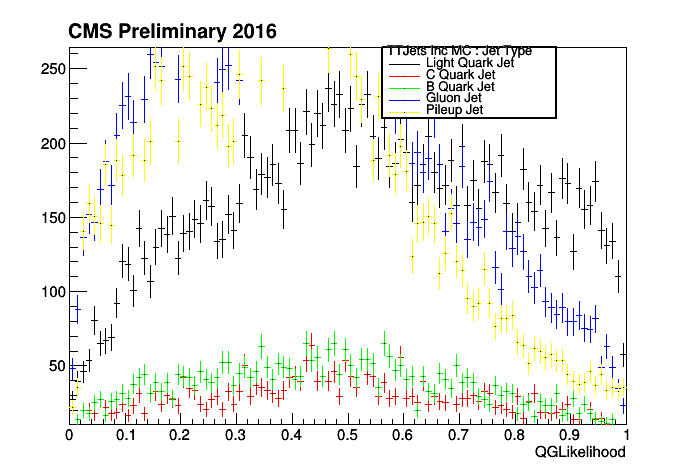
\includegraphics[width=0.45\textwidth]{sections/mc4/TopTagger/figures/_b_qglikelihoodjetetabin3_.png} \\
  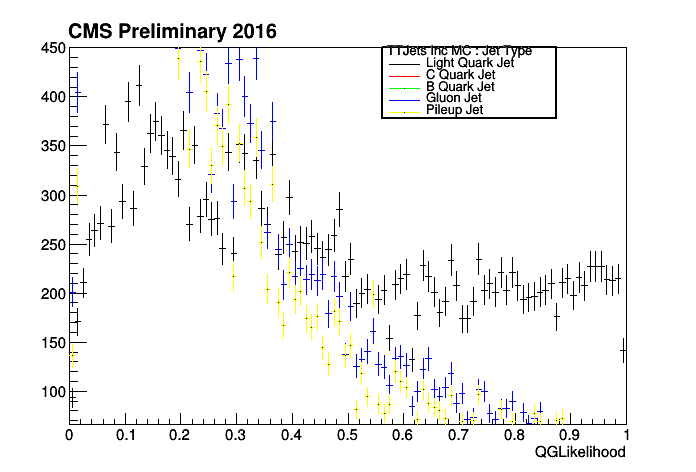
\includegraphics[width=0.45\textwidth]{sections/mc4/TopTagger/figures/_b_qglikelihoodjetetabin4_.png}
  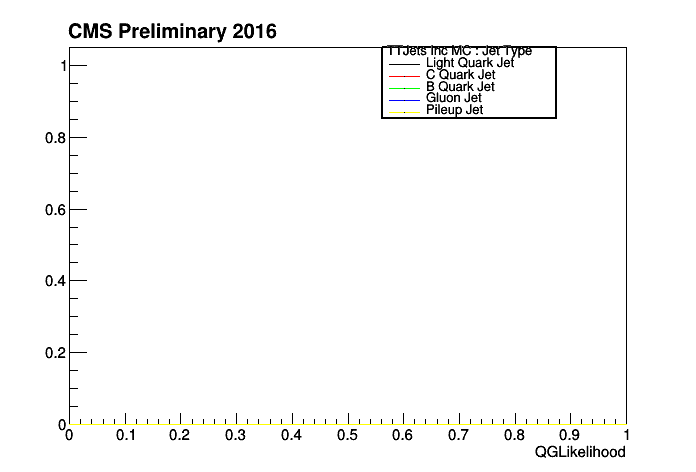
\includegraphics[width=0.45\textwidth]{sections/mc4/TopTagger/figures/_b_qglikelihoodjetetabin5_.png}
 \end{center}
 \caption{Top left: Quark Gluon likelihood for jet $\eta$ bin 1; Top right: jet $\eta$ bin 2; Middle left: jet $\eta$ bin 3; Middle right: jet $\eta$ bin 4; Middle left: jet $\eta$ bin 5; Middle right: jet $\eta$ bin 6}
 \label{fig:c4ttqgljeteta}
\end{figure}

The performance in terms of jet $p_{T}$ in different jet flavors is shown in Fig~\ref{fig:c4ttqgljetpt}. The discrimination power for HEHF and HF jets is not ideal.
\begin{figure}[htbp]
 \begin{center}
  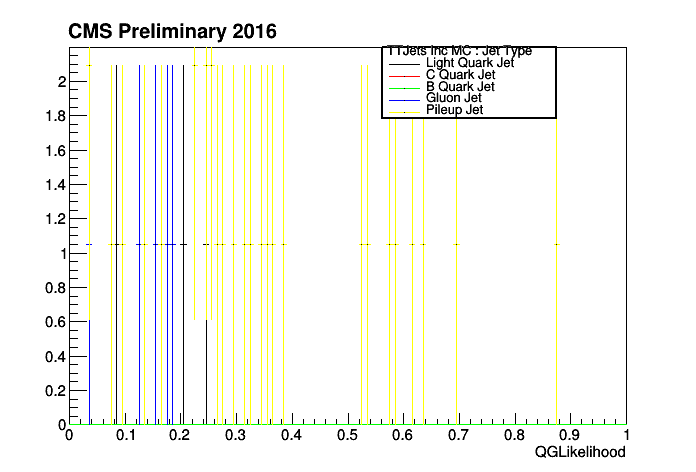
\includegraphics[width=0.45\textwidth]{sections/mc4/TopTagger/figures/_b_qglikelihoodjetptbin0_.png}
  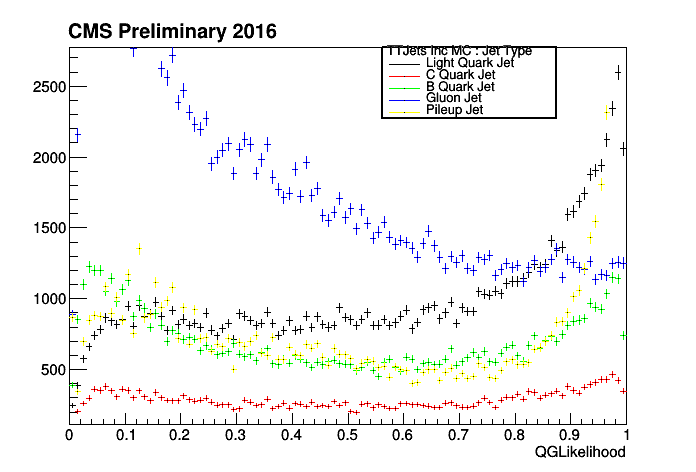
\includegraphics[width=0.45\textwidth]{sections/mc4/TopTagger/figures/_b_qglikelihoodjetptbin1_.png} \\
  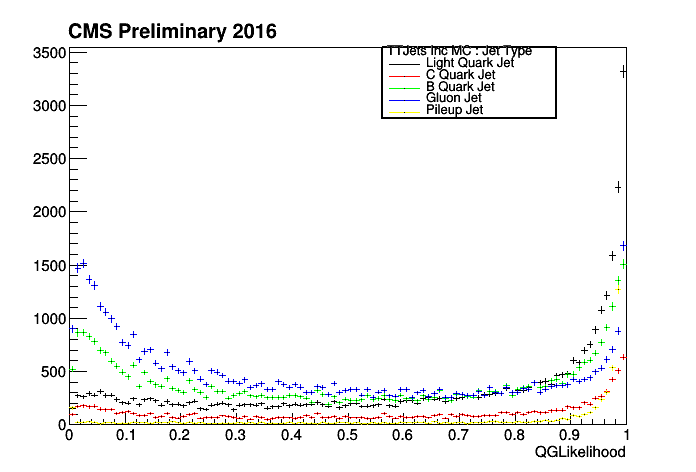
\includegraphics[width=0.45\textwidth]{sections/mc4/TopTagger/figures/_b_qglikelihoodjetptbin2_.png} 
  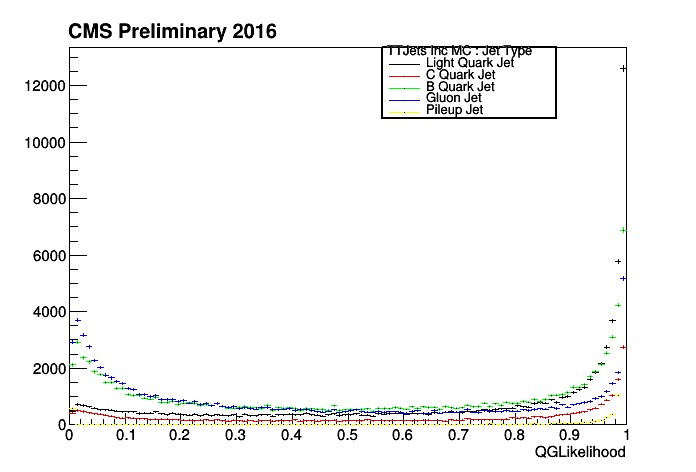
\includegraphics[width=0.45\textwidth]{sections/mc4/TopTagger/figures/_b_qglikelihoodjetptbin3_.png} \\
  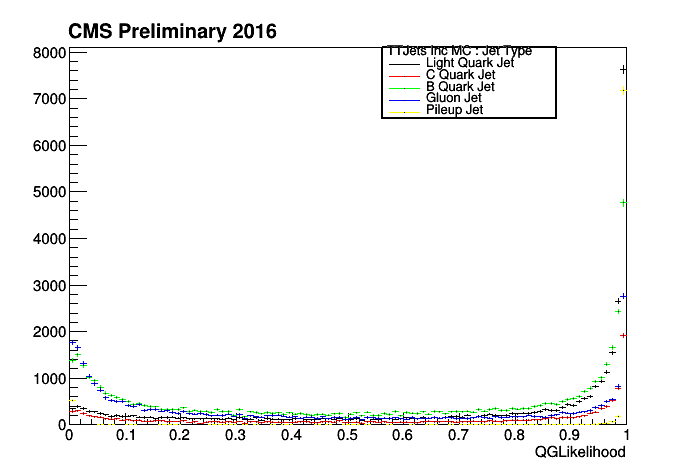
\includegraphics[width=0.45\textwidth]{sections/mc4/TopTagger/figures/_b_qglikelihoodjetptbin4_.png}
  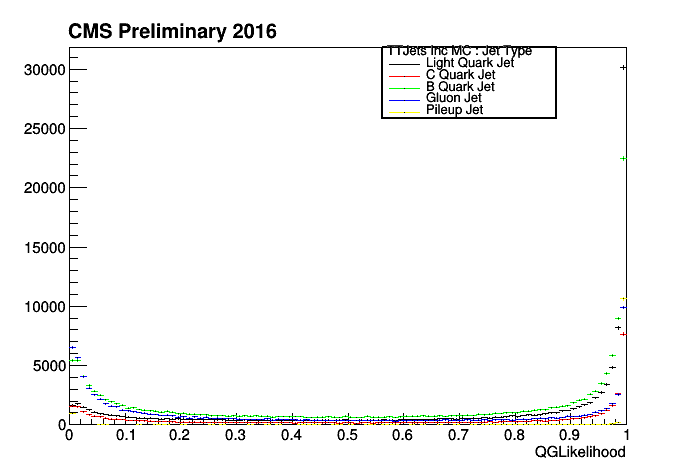
\includegraphics[width=0.45\textwidth]{sections/mc4/TopTagger/figures/_b_qglikelihoodjetptbin5_.png}
 \end{center}
 \caption{Top left: Quark Gluon likelihood for jet $p_{T}$ bin 1; Top right: jet $p_{T}$ bin 2; Middle left: jet $p_{T}$ bin 3; Middle right: jet $p_{T}$ bin 4; Middle left: jet $p_{T}$ bin 5; Middle right: jet $p_{T}$ bin 6}
 \label{fig:c4ttqgljetpt}
\end{figure}

The quark gluon discriminator does not work well for b-jet in all cases. Therefore, for tagged b jets, the likelihood is set equal to 1 (quark jet) before being trained.

All the variables are fed into the random forest\cite{Ho:1995:RDF:844379.844681} training algorithm for training in simulation samples. We designed three points, each with a different balance of reconstruction efficiency versus mistag rate. In the end, we chose the tight working point for the analysis, based on the results of sensitivity studies. The combined top-jet reconstruction efficiency (Fig~\ref{fig:c4ttefftight}) is about 60\%. The mistag rate (Fig~\ref{fig:c4ttmistagtight}) is around 20\%, which is about a factor of two smaller than for the cut-based top tagger used in the analysis of the 2015 data. Additional studies were performed to study the difference between the performance of the top tagger in the full simulation and data, and also between the full simulation and fast simulation, since we use the fast simulation for limit setting. Scale factors that account for differences between the data and full simulation, or between the fast and full simulation, in the top tagger performance, are binned in the top quark $p_{T}$ and applied to the data before limit setting. More details are given in Ref.\cite{AN-16-461}. 

\begin{figure}[htbp]
 \begin{center}
  %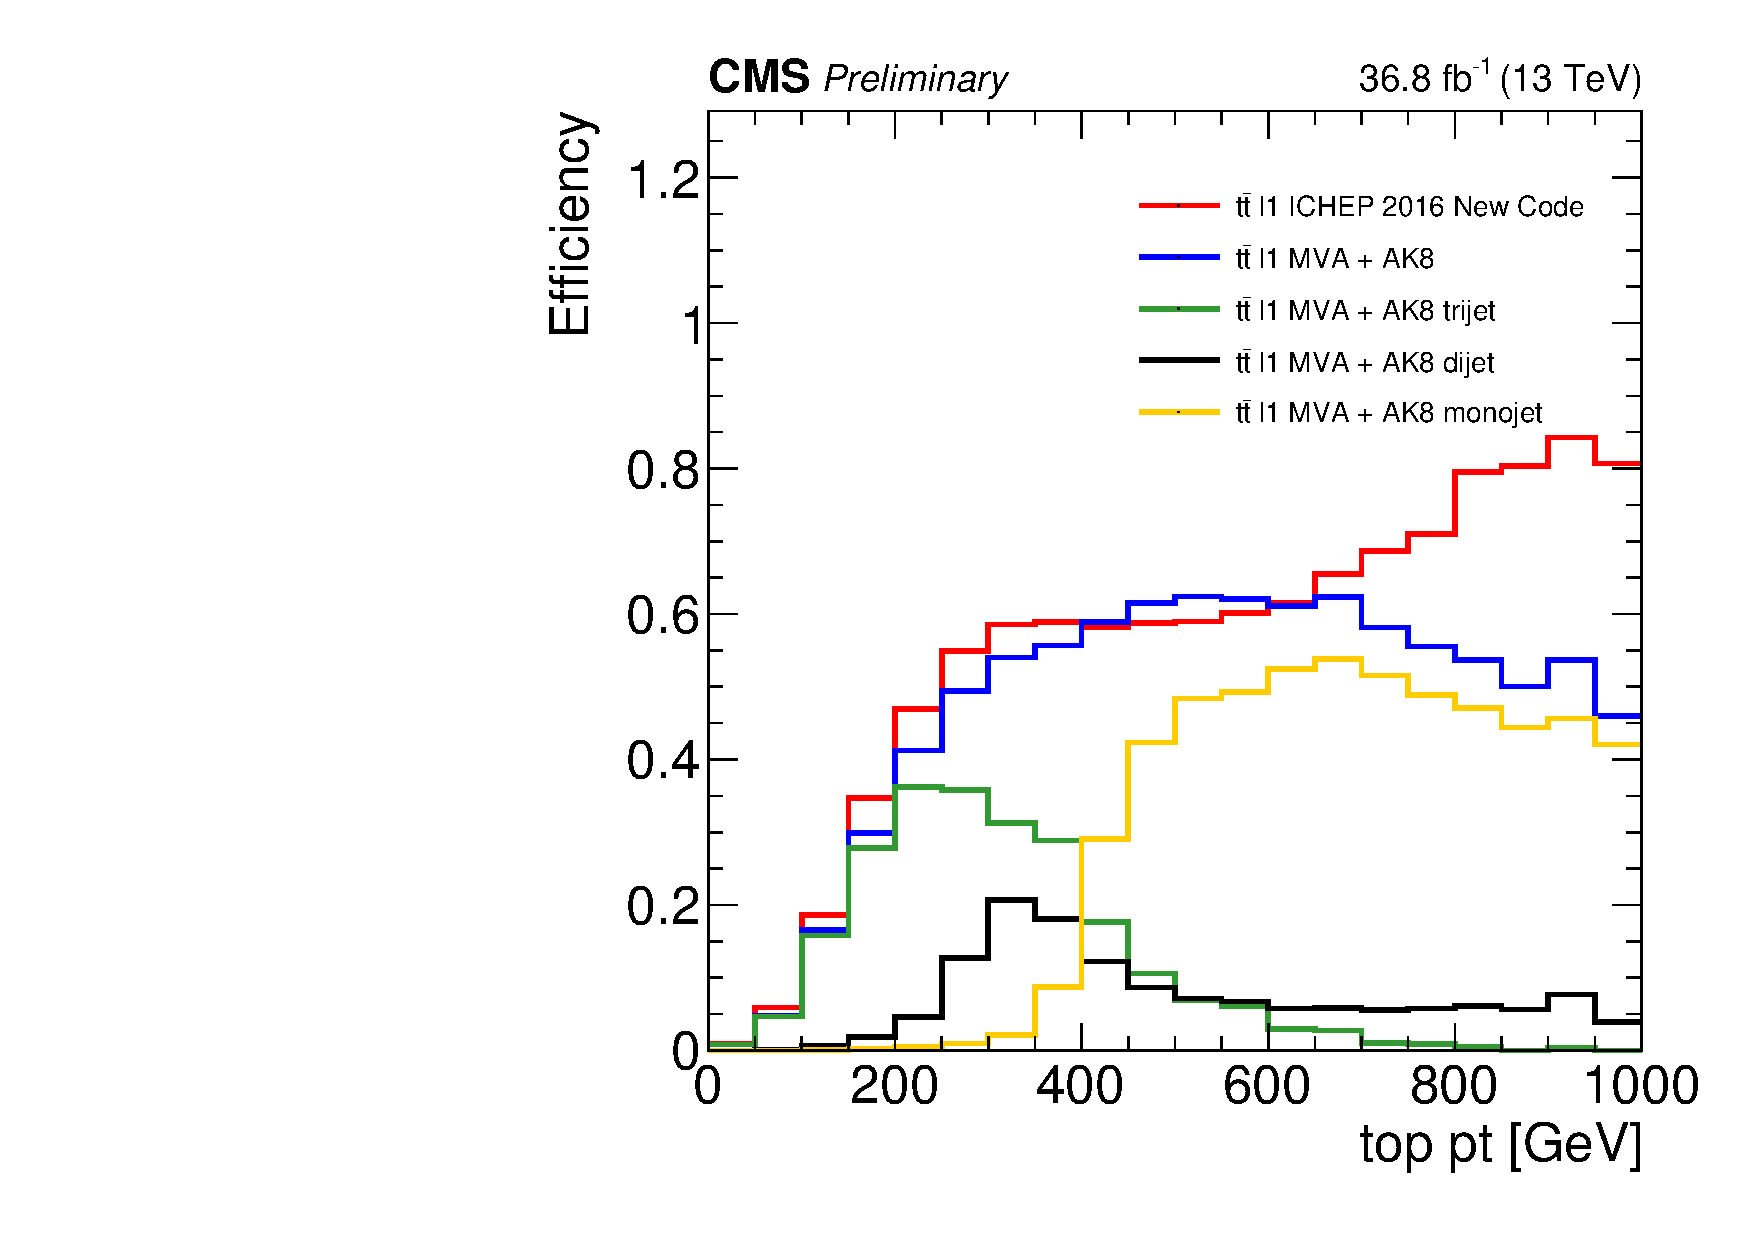
\includegraphics[width=0.90\textwidth]{sections/mc4/TopTagger/figures/baseline_eff_pt_ttbar1l_tight.pdf}
  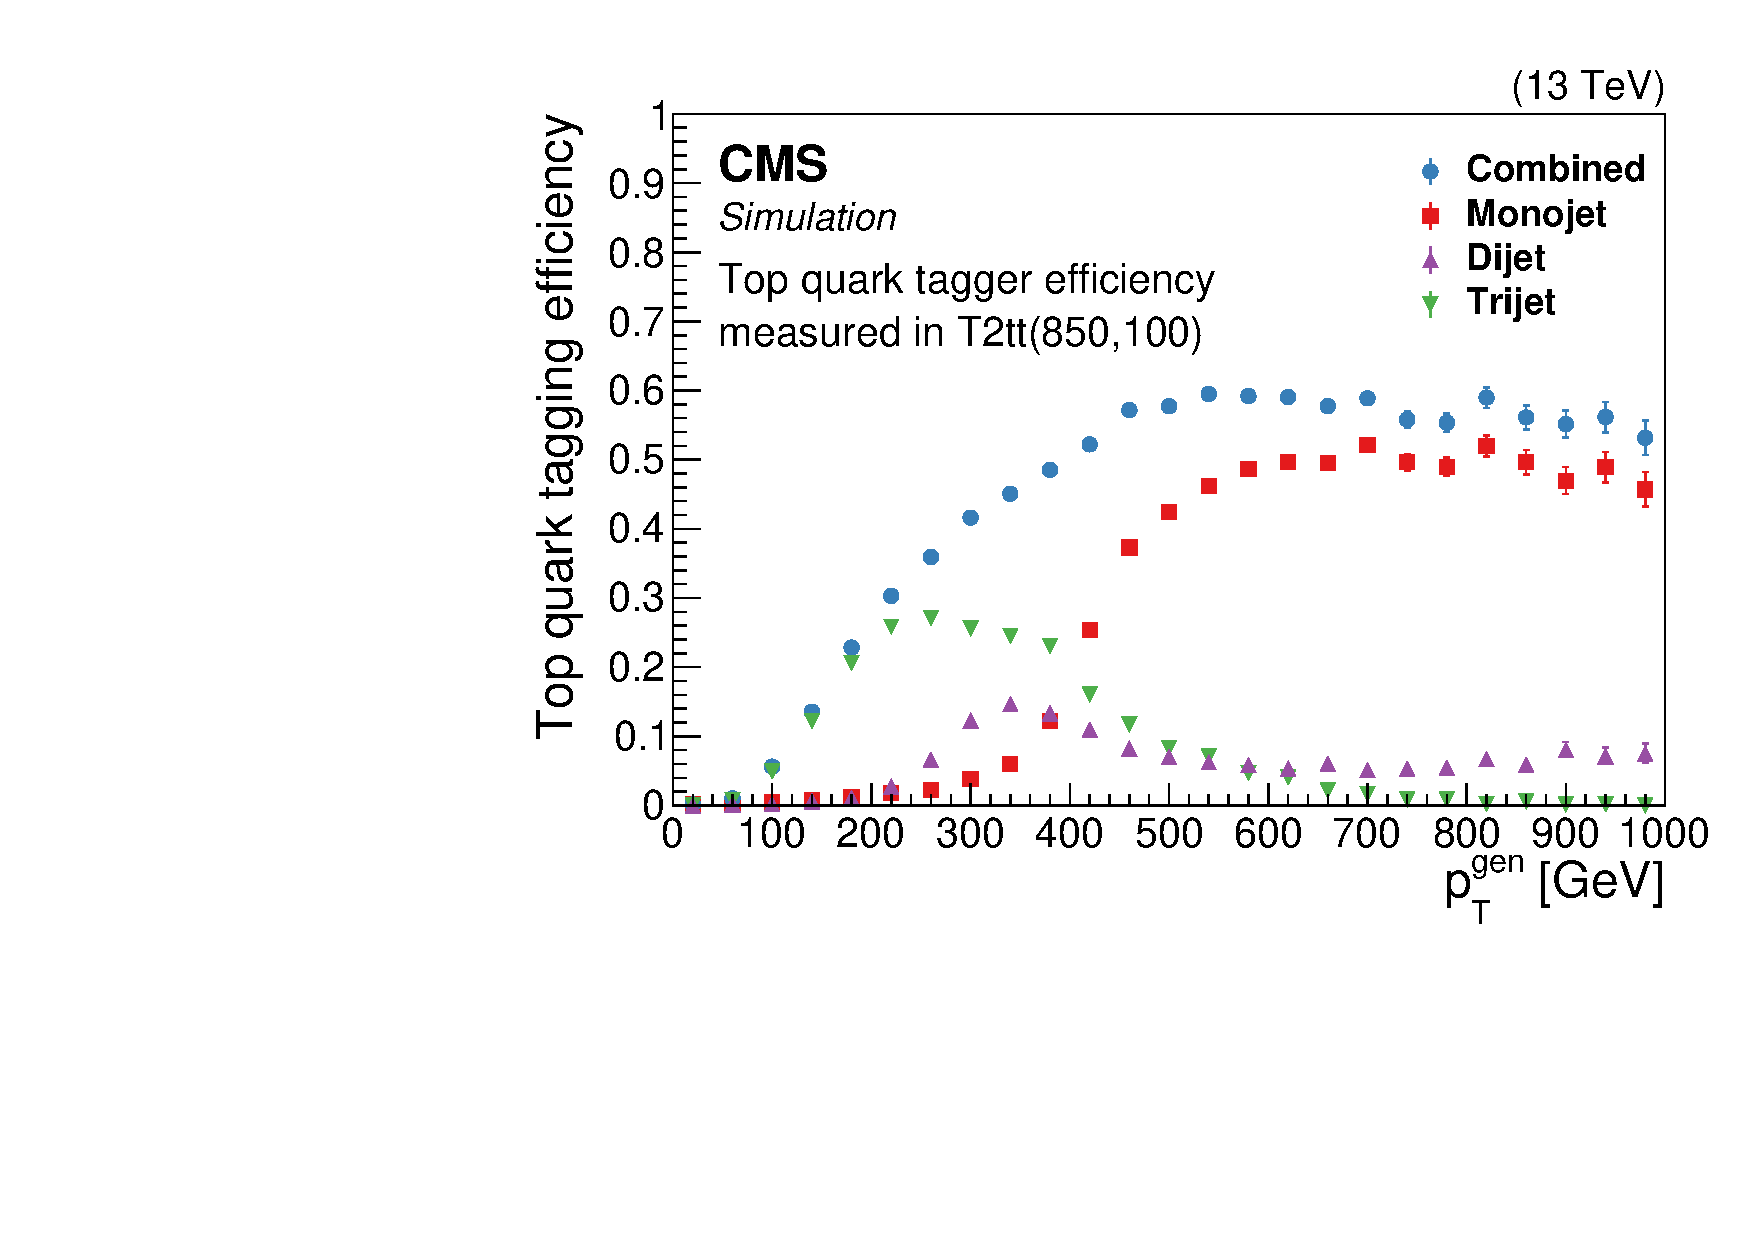
\includegraphics[width=0.90\textwidth]{sections/mc4/TopTagger/figures/Tagger_Paper.pdf}
 \end{center}
 \caption{Efficiency of the top quark tagger as a function of generator-level top quark $p_{T}$ for
the monojet (red boxes), dijet (magenta upper-triangles), and trijet (green lower-triangles) categories
and for their combination (blue circles), as determined using T2tt signal events with a
top squark mass of 850 GeV and an LSP mass of 100 GeV. The vertical bars indicate the statistical
uncertainties.}
 \label{fig:c4ttefftight}
\end{figure}

\begin{figure}[htbp]
 \begin{center}
  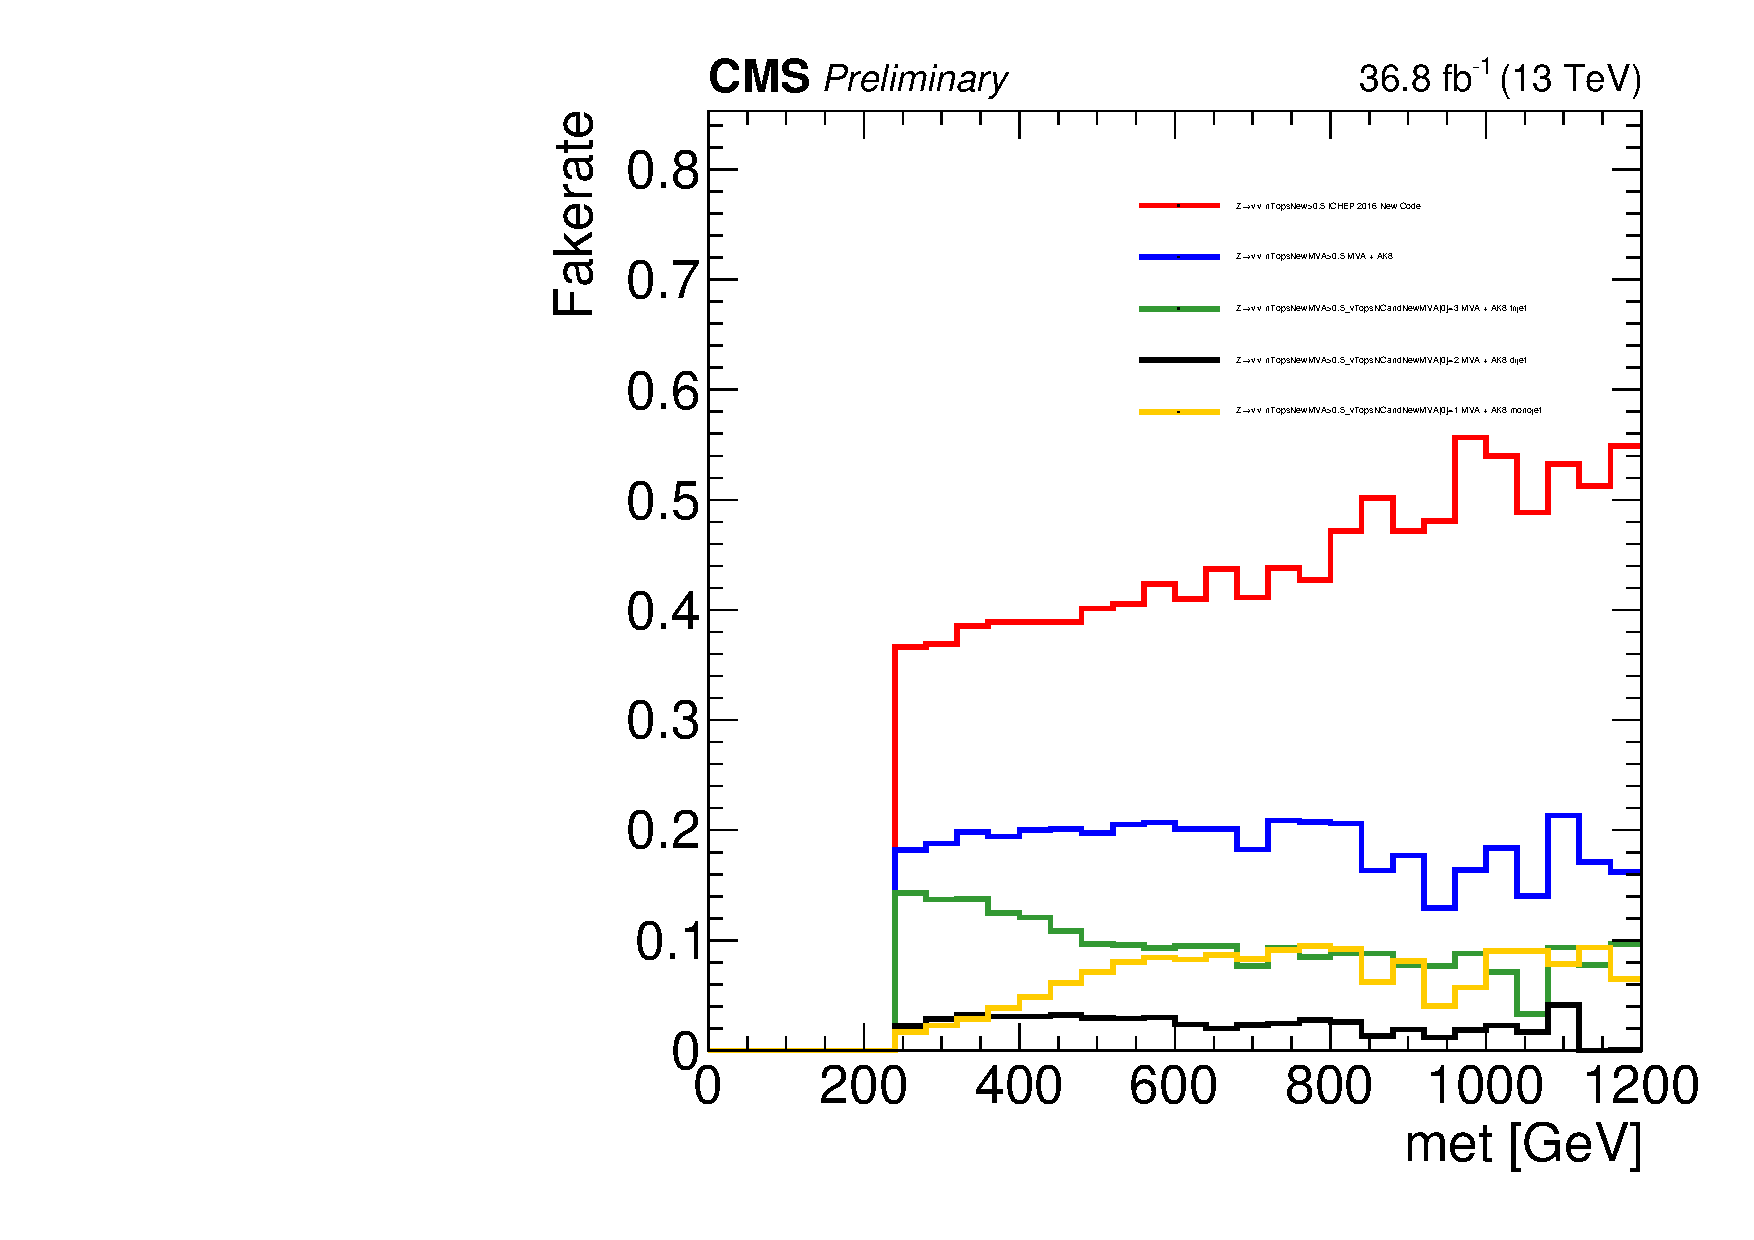
\includegraphics[width=0.45\textwidth]{sections/mc4/TopTagger/figures/baseline_fakerate_met_tight.pdf}
  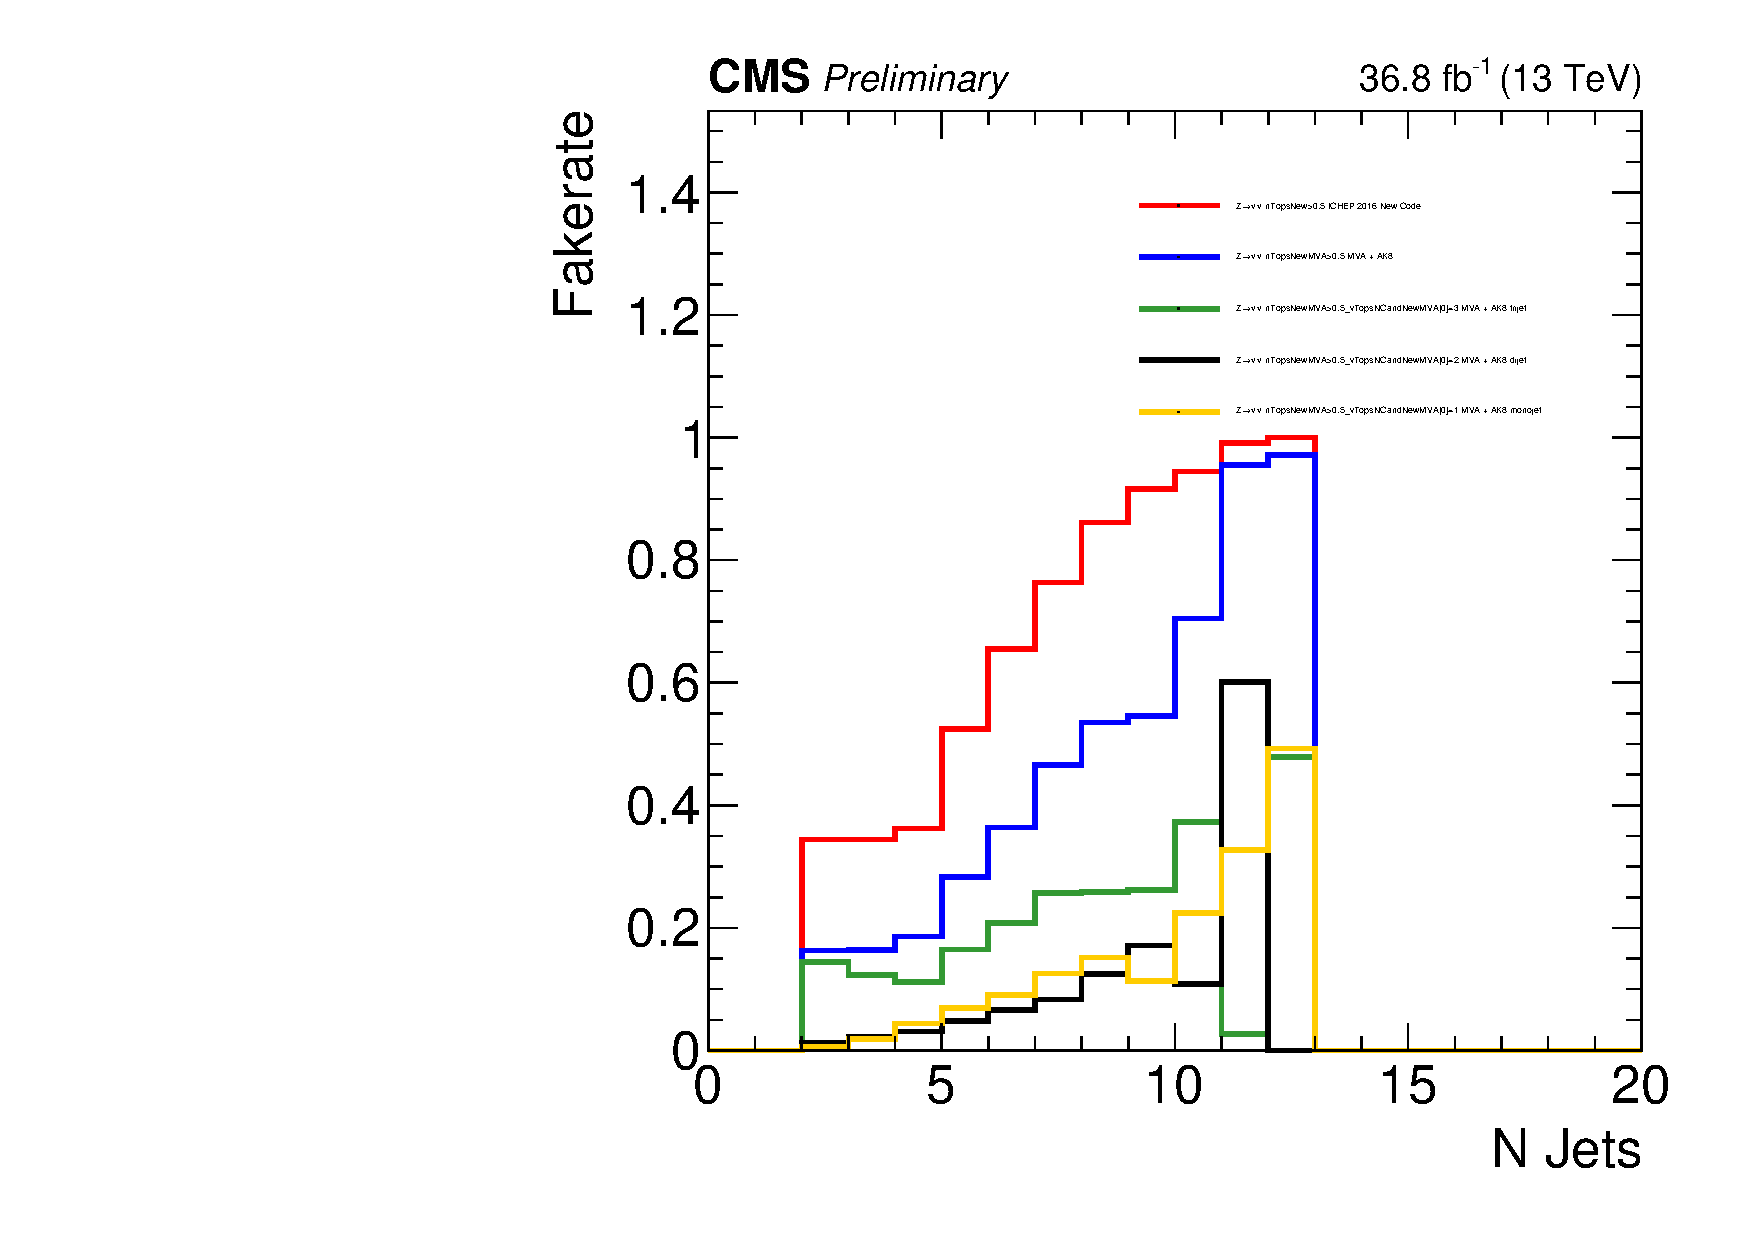
\includegraphics[width=0.45\textwidth]{sections/mc4/TopTagger/figures/baseline_fakerate_njet_tight.pdf}
 \end{center} \caption{Top-jet reconstruction mistag rate, measured in $Z$+jets simulation samples. Left plot is the distribution in \MET, Right plot is in \njets. The red curve is the mistag rate for cut-based top tagger, the blue curve is the mistag rate for multivariate top tagger. The green, black and yellow are the mistag rate for tri-jet, di-jet and mono-jet, respectively.}
 \label{fig:c4ttmistagtight}
\end{figure}
